\documentclass{standalone}
\usepackage{tikz}
\usetikzlibrary{patterns, positioning}

\begin{document}
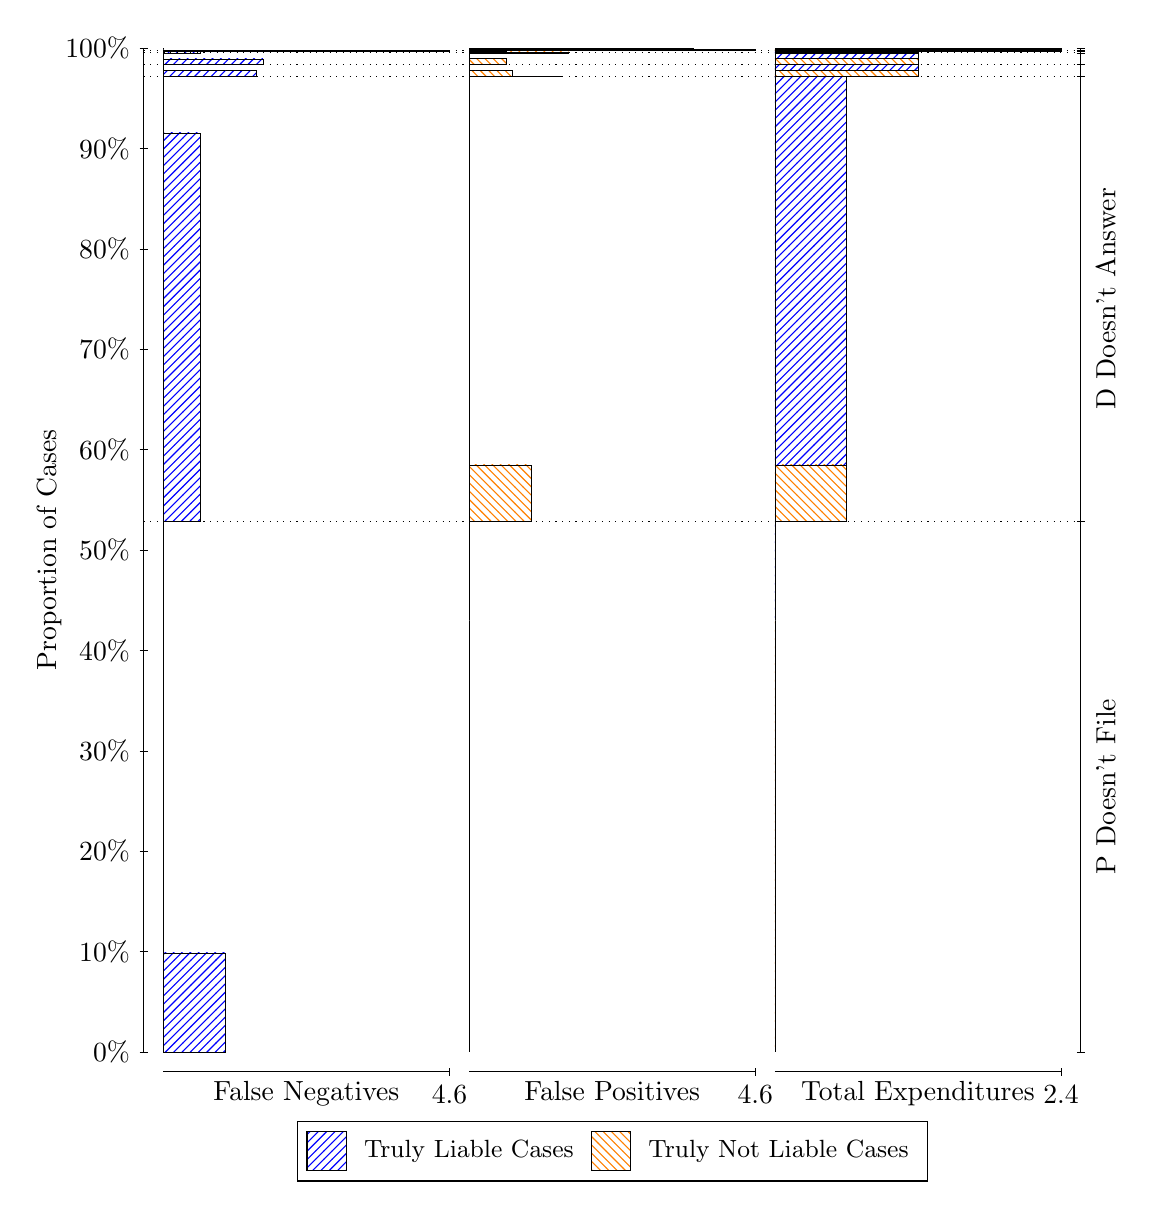
\begin{tikzpicture}
\draw[black, very thin] (1.5,1.75) -- (1.5,14.5);
\node[rotate=90, anchor=center] at (0.3, 8.125) {Proportion of Cases};
\draw[black, very thin] (1.45,1.75) -- (1.55,1.75);
\node[anchor=east] at (1.45, 1.75) {0\%};
\draw[black, very thin] (1.45,3.025) -- (1.55,3.025);
\node[anchor=east] at (1.45, 3.025) {10\%};
\draw[black, very thin] (1.45,4.3) -- (1.55,4.3);
\node[anchor=east] at (1.45, 4.3) {20\%};
\draw[black, very thin] (1.45,5.575) -- (1.55,5.575);
\node[anchor=east] at (1.45, 5.575) {30\%};
\draw[black, very thin] (1.45,6.85) -- (1.55,6.85);
\node[anchor=east] at (1.45, 6.85) {40\%};
\draw[black, very thin] (1.45,8.125) -- (1.55,8.125);
\node[anchor=east] at (1.45, 8.125) {50\%};
\draw[black, very thin] (1.45,9.4) -- (1.55,9.4);
\node[anchor=east] at (1.45, 9.4) {60\%};
\draw[black, very thin] (1.45,10.675) -- (1.55,10.675);
\node[anchor=east] at (1.45, 10.675) {70\%};
\draw[black, very thin] (1.45,11.95) -- (1.55,11.95);
\node[anchor=east] at (1.45, 11.95) {80\%};
\draw[black, very thin] (1.45,13.225) -- (1.55,13.225);
\node[anchor=east] at (1.45, 13.225) {90\%};
\draw[black, very thin] (1.45,14.5) -- (1.55,14.5);
\node[anchor=east] at (1.45, 14.5) {100\%};

\draw[black, very thin] (13.4,1.75) -- (13.4,14.5);
\draw[black, very thin] (13.35,1.75) -- (13.45,1.75);
\node[anchor=west] at (13.35, 1.75) {};
\draw[black, very thin] (13.35,8.4878) -- (13.45,8.4878);
\node[anchor=west] at (13.35, 8.4878) {};
\draw[black, very thin] (13.35,14.139) -- (13.45,14.139);
\node[anchor=west] at (13.35, 14.139) {};
\draw[black, very thin] (13.35,14.29) -- (13.45,14.29);
\node[anchor=west] at (13.35, 14.29) {};
\draw[black, very thin] (13.35,14.438) -- (13.45,14.438);
\node[anchor=west] at (13.35, 14.438) {};
\draw[black, very thin] (13.35,14.465) -- (13.45,14.465);
\node[anchor=west] at (13.35, 14.465) {};
\draw[black, very thin] (13.35,14.473) -- (13.45,14.473);
\node[anchor=west] at (13.35, 14.473) {};
\draw[black, very thin] (13.35,14.5) -- (13.45,14.5);
\node[anchor=west] at (13.35, 14.5) {};

\draw[black, very thin, pattern color=blue, pattern=north east lines] (1.75,1.75) rectangle (2.5399,3.0093);
\draw[black, very thin, pattern color=orange, pattern=north west lines] (1.75,3.0093) rectangle (1.75,8.4878);
\draw[black, very thin, pattern color=blue, pattern=north east lines] (1.75,8.4878) rectangle (2.2239,13.421);
\draw[black, very thin, pattern color=orange, pattern=north west lines] (1.75,13.421) rectangle (1.75,14.139);
\draw[black, very thin, pattern color=blue, pattern=north east lines] (1.75,14.139) rectangle (2.9348,14.212);
\draw[black, very thin, pattern color=blue, pattern=north east lines] (1.75,14.212) rectangle (2.8558,14.212);
\draw[black, very thin, pattern color=blue, pattern=north east lines] (1.75,14.212) rectangle (2.7768,14.212);
\draw[black, very thin, pattern color=blue, pattern=north east lines] (1.75,14.212) rectangle (2.6978,14.212);
\draw[black, very thin, pattern color=blue, pattern=north east lines] (1.75,14.212) rectangle (2.6188,14.212);
\draw[black, very thin, pattern color=blue, pattern=north east lines] (1.75,14.212) rectangle (2.5399,14.212);
\draw[black, very thin, pattern color=blue, pattern=north east lines] (1.75,14.212) rectangle (2.4609,14.212);
\draw[black, very thin, pattern color=blue, pattern=north east lines] (1.75,14.212) rectangle (2.3819,14.212);
\draw[black, very thin, pattern color=blue, pattern=north east lines] (1.75,14.212) rectangle (2.3029,14.212);
\draw[black, very thin, pattern color=orange, pattern=north west lines] (1.75,14.212) rectangle (1.75,14.29);
\draw[black, very thin, pattern color=blue, pattern=north east lines] (1.75,14.29) rectangle (3.0138,14.361);
\draw[black, very thin, pattern color=orange, pattern=north west lines] (1.75,14.361) rectangle (1.75,14.438);
\draw[black, very thin, pattern color=blue, pattern=north east lines] (1.75,14.438) rectangle (2.2239,14.453);
\draw[black, very thin, pattern color=orange, pattern=north west lines] (1.75,14.453) rectangle (1.75,14.465);
\draw[black, very thin, pattern color=blue, pattern=north east lines] (1.75,14.465) rectangle (5.3833,14.469);
\draw[black, very thin, pattern color=orange, pattern=north west lines] (1.75,14.469) rectangle (1.75,14.473);
\draw[black, very thin, pattern color=orange, pattern=north west lines] (1.75,14.473) rectangle (1.75,14.481);
\draw[black, very thin, pattern color=blue, pattern=north east lines] (1.75,14.481) rectangle (1.75,14.5);
\draw[black, very thin, pattern color=orange, pattern=north west lines] (5.6333,1.75) rectangle (5.6333,7.2285);
\draw[black, very thin, pattern color=blue, pattern=north east lines] (5.6333,7.2285) rectangle (5.6333,8.4878);
\draw[black, very thin, pattern color=orange, pattern=north west lines] (5.6333,8.4878) rectangle (6.4232,9.2057);
\draw[black, very thin, pattern color=blue, pattern=north east lines] (5.6333,9.2057) rectangle (5.6333,14.139);
\draw[black, very thin, pattern color=orange, pattern=north west lines] (5.6333,14.139) rectangle (6.8181,14.139);
\draw[black, very thin, pattern color=orange, pattern=north west lines] (5.6333,14.139) rectangle (6.7391,14.139);
\draw[black, very thin, pattern color=orange, pattern=north west lines] (5.6333,14.139) rectangle (6.6601,14.139);
\draw[black, very thin, pattern color=orange, pattern=north west lines] (5.6333,14.139) rectangle (6.5812,14.139);
\draw[black, very thin, pattern color=orange, pattern=north west lines] (5.6333,14.139) rectangle (6.5022,14.139);
\draw[black, very thin, pattern color=orange, pattern=north west lines] (5.6333,14.139) rectangle (6.4232,14.139);
\draw[black, very thin, pattern color=orange, pattern=north west lines] (5.6333,14.139) rectangle (6.3442,14.139);
\draw[black, very thin, pattern color=orange, pattern=north west lines] (5.6333,14.139) rectangle (6.2652,14.139);
\draw[black, very thin, pattern color=orange, pattern=north west lines] (5.6333,14.139) rectangle (6.1862,14.217);
\draw[black, very thin, pattern color=blue, pattern=north east lines] (5.6333,14.217) rectangle (6.0283,14.217);
\draw[black, very thin, pattern color=blue, pattern=north east lines] (5.6333,14.217) rectangle (5.9493,14.217);
\draw[black, very thin, pattern color=blue, pattern=north east lines] (5.6333,14.217) rectangle (5.8703,14.217);
\draw[black, very thin, pattern color=blue, pattern=north east lines] (5.6333,14.217) rectangle (5.7913,14.217);
\draw[black, very thin, pattern color=blue, pattern=north east lines] (5.6333,14.217) rectangle (5.7123,14.217);
\draw[black, very thin, pattern color=blue, pattern=north east lines] (5.6333,14.217) rectangle (5.6333,14.29);
\draw[black, very thin, pattern color=orange, pattern=north west lines] (5.6333,14.29) rectangle (6.1072,14.367);
\draw[black, very thin, pattern color=blue, pattern=north east lines] (5.6333,14.367) rectangle (5.6333,14.438);
\draw[black, very thin, pattern color=orange, pattern=north west lines] (5.6333,14.438) rectangle (6.8971,14.45);
\draw[black, very thin, pattern color=blue, pattern=north east lines] (5.6333,14.45) rectangle (6.1072,14.465);
\draw[black, very thin, pattern color=orange, pattern=north west lines] (5.6333,14.465) rectangle (5.6333,14.469);
\draw[black, very thin, pattern color=blue, pattern=north east lines] (5.6333,14.469) rectangle (5.6333,14.473);
\draw[black, very thin, pattern color=orange, pattern=north west lines] (5.6333,14.473) rectangle (9.2667,14.481);
\draw[black, very thin, pattern color=blue, pattern=north east lines] (5.6333,14.481) rectangle (8.4768,14.5);
\draw[black, very thin, pattern color=orange, pattern=north west lines] (9.5167,1.75) rectangle (9.5167,7.2285);
\draw[black, very thin, pattern color=blue, pattern=north east lines] (9.5167,7.2285) rectangle (9.5167,8.4878);
\draw[black, very thin, pattern color=orange, pattern=north west lines] (9.5167,8.4878) rectangle (10.425,9.2057);
\draw[black, very thin, pattern color=blue, pattern=north east lines] (9.5167,9.2057) rectangle (10.425,14.139);
\draw[black, very thin, pattern color=orange, pattern=north west lines] (9.5167,14.139) rectangle (11.333,14.139);
\draw[black, very thin, pattern color=blue, pattern=north east lines] (9.5167,14.139) rectangle (11.333,14.139);
\draw[black, very thin, pattern color=orange, pattern=north west lines] (9.5167,14.139) rectangle (11.333,14.217);
\draw[black, very thin, pattern color=blue, pattern=north east lines] (9.5167,14.217) rectangle (11.333,14.29);
\draw[black, very thin, pattern color=orange, pattern=north west lines] (9.5167,14.29) rectangle (11.333,14.29);
\draw[black, very thin, pattern color=blue, pattern=north east lines] (9.5167,14.29) rectangle (11.333,14.29);
\draw[black, very thin, pattern color=orange, pattern=north west lines] (9.5167,14.29) rectangle (11.333,14.367);
\draw[black, very thin, pattern color=blue, pattern=north east lines] (9.5167,14.367) rectangle (11.333,14.438);
\draw[black, very thin, pattern color=orange, pattern=north west lines] (9.5167,14.438) rectangle (11.333,14.45);
\draw[black, very thin, pattern color=blue, pattern=north east lines] (9.5167,14.45) rectangle (11.333,14.465);
\draw[black, very thin, pattern color=orange, pattern=north west lines] (9.5167,14.465) rectangle (13.15,14.469);
\draw[black, very thin, pattern color=blue, pattern=north east lines] (9.5167,14.469) rectangle (13.15,14.473);
\draw[black, very thin, pattern color=orange, pattern=north west lines] (9.5167,14.473) rectangle (13.15,14.481);
\draw[black, very thin, pattern color=blue, pattern=north east lines] (9.5167,14.481) rectangle (13.15,14.5);
\draw[black, dotted] (1.5,8.4878) -- (13.4,8.4878);
\draw[black, dotted] (1.5,14.139) -- (13.4,14.139);
\draw[black, dotted] (1.5,14.29) -- (13.4,14.29);
\draw[black, dotted] (1.5,14.438) -- (13.4,14.438);
\draw[black, dotted] (1.5,14.465) -- (13.4,14.465);
\draw[black, dotted] (1.5,14.473) -- (13.4,14.473);
\draw[black, very thin] (1.75,1.5) -- (5.3833,1.5);
\node[anchor=north] at (3.5667, 1.5) {False Negatives};
\draw[black, very thin] (5.3833,1.45) -- (5.3833,1.55);
\node[anchor=north] at (5.3833, 1.45) {4.6};

\draw[black, very thin] (5.6333,1.5) -- (9.2667,1.5);
\node[anchor=north] at (7.45, 1.5) {False Positives};
\draw[black, very thin] (9.2667,1.45) -- (9.2667,1.55);
\node[anchor=north] at (9.2667, 1.45) {4.6};

\draw[black, very thin] (9.5167,1.5) -- (13.15,1.5);
\node[anchor=north] at (11.333, 1.5) {Total Expenditures};
\draw[black, very thin] (13.15,1.45) -- (13.15,1.55);
\node[anchor=north] at (13.15, 1.45) {2.4};

\node[black, centered, rotate=90] at (13.72, 5.1189) {P Doesn't File};
\node[black, centered, rotate=90] at (13.72, 11.313) {D Doesn't Answer};






\draw (7.449999999999999,1.5) node[draw=none] (baseCoordinate) {};
\begin{scope}[align=center]
        \matrix[scale=0.5, draw=black, below=0.5cm of baseCoordinate, nodes={draw}, column sep=0.1cm]{
            \node[rectangle, draw, minimum width=0.5cm, minimum height=0.5cm, pattern=north east lines, pattern color=blue] {}; &
            \node[draw=none, font=\small] (B) {Truly Liable Cases}; &
            \node[rectangle, draw, minimum width=0.5cm, minimum height=0.5cm, pattern=north west lines, pattern color=orange] {}; &
            \node[draw=none, font=\small] (B) {Truly Not Liable Cases}; \\
            };
\end{scope}

\end{tikzpicture}
\end{document}